%\documentclass[handout]{beamer}
\documentclass[public]{beamer}
\usepackage{econtexShortcuts}%\usepackage{econtexSetup}
\usepackage{ifthen}
\usepackage{verbatim}

% Create tools to allow this document to generate different versions (e.g., NBER, or Fed) depending on flags
\provideboolean{includeFrameTF}\setboolean{includeFrameTF}{true} % Default is to include 
\provideboolean{includeTextTF}\setboolean{includeTextTF}{true} % 
\provideboolean{includeTF}\setboolean{includeTF}{true} % 

% \newcommand{\ifAnswers}{\ifthenelse{\boolean{includeTF}}}
\newcommand{\ifIncludeFrame}[1]{\ifthenelse{\boolean{includeFrameTF}}{#1}}
\newcommand{\ifIncludeText}[1]{\ifthenelse{\boolean{includeTextTF}}{#1}}
\newcommand{\ifInclude}[1]{\ifthenelse{\boolean{includeTF}}{#1}}

\usetheme{Madrid}
\definecolor{orange}{HTML}{FF7F00}\hypersetup{colorlinks,linkcolor=,urlcolor=orange}

% Redefine footer from
% http://tex.stackexchange.com/questions/83048/change-the-contents-of-footline-in-a-beamer-presentation
\setbeamertemplate{footline}
{
  \leavevmode%
  \hbox{%
    \begin{beamercolorbox}[wd=.333333\paperwidth,ht=2.25ex,dp=1ex,center]{author in head/foot}%
      \usebeamerfont{author in head/foot}\insertsection
    \end{beamercolorbox}%
    \begin{beamercolorbox}[wd=.333333\paperwidth,ht=2.25ex,dp=1ex,center]{title in head/foot}%
      \usebeamerfont{title in head/foot}\insertsubsection
    \end{beamercolorbox}%
    \begin{beamercolorbox}[wd=.333333\paperwidth,ht=2.25ex,dp=1ex,right]{date in head/foot}%
      \usebeamerfont{date in head/foot}\insertshortdate{}\hspace*{2em}
      \insertframenumber{} / \inserttotalframenumber\hspace*{2ex} 
    \end{beamercolorbox}}%
  \vskip0pt%
}
\makeatother

\providecommand{\EconARK}{\href{http://econ-ark.org}{econ-ark.org}}

\providecommand{\CDC}{\texttt{CDC}}
\providecommand{\NMP}{\texttt{NMP}}
\providecommand{\MNW}{\texttt{MNW}}
\providecommand{\DCL}{\texttt{DCL}}
\providecommand{\JXY}{\texttt{JXY}}
\providecommand{\ABK}{\texttt{ABK}}


\provideboolean{CESifo}
\setboolean{CESifo}{true}
% \setboolean{CESifo}{false}
\providecommand{\CESifoYN}{\ifthenelse{\boolean{CESifo}}}

\provideboolean{PARKmake}
\setboolean{PARKmake}{true}
% \setboolean{PARKmake}{false}
\providecommand{\PARKmakeYN}{\ifthenelse{\boolean{PARKmake}}}

\provideboolean{NBERMtoM}
\setboolean{NBERMtoM}{true}
% \setboolean{NBERMtoM}{false}
\providecommand{\NBERMtoMYN}{\ifthenelse{\boolean{NBERMtoM}}}

\provideboolean{GMU}
\setboolean{GMU}{true}
\setboolean{GMU}{false}
\providecommand{\GMUYN}{\ifthenelse{\boolean{GMU}}}

\provideboolean{ECB}
\setboolean{ECB}{true}
\setboolean{ECB}{false}
\providecommand{\ECBYN}{\ifthenelse{\boolean{ECB}}}

\provideboolean{Elt} % Eltville Bundesbank conference
\setboolean{Elt}{true}
\setboolean{Elt}{false}
\providecommand{\EltYN}{\ifthenelse{\boolean{Elt}}}

\provideboolean{SAFE} % Goethe/SAFE
\setboolean{SAFE}{true}
\setboolean{SAFE}{false}
\providecommand{\SAFEYN}{\ifthenelse{\boolean{SAFE}}}

\provideboolean{BoE} % Bank of England, 2018-06-04 and 06
\setboolean{BoE}{true}
% \setboolean{BoE}{false}
\providecommand{\BoEYN}{\ifthenelse{\boolean{BoE}}}

\providecommand{\PARKmakeHideTextBegin}{\ifthenelse{\boolean{PARKmake}}{\setboolean{includeTextTF}{false}}{}}
\providecommand{\PARKmakeHideTextEnd}{  \ifthenelse{\boolean{PARKmake}}{\setboolean{includeTextTF}{true}}{}}

\providecommand{\PARKmakeHideFrameBegin}{\ifthenelse{\boolean{PARKmake}}{\setboolean{includeFrameTF}{false}}{}}
\providecommand{\PARKmakeHideFrameEnd}{  \ifthenelse{\boolean{PARKmake}}{\setboolean{includeFrameTF}{true}}{}}

\providecommand{\PARKmakeHideBegin}{\ifthenelse{\boolean{PARKmake}}{\setboolean{includeTF}{false}}{}}
\providecommand{\PARKmakeHideEnd}{  \ifthenelse{\boolean{PARKmake}}{\setboolean{includeTF}{true}}{}}

\providecommand{\NBERMtoMHideBegin}{\ifthenelse{\boolean{NBERMtoM}}{\setboolean{includeTF}{false}}{}}
\providecommand{\NBERMtoMHideEnd}{  \ifthenelse{\boolean{NBERMtoM}}{\setboolean{includeTF}{true}}{}}

\providecommand{\GMUHideBegin}{\ifthenelse{\boolean{GMU}}{\setboolean{includeTF}{false}}{}}
\providecommand{\GMUHideEnd}{  \ifthenelse{\boolean{GMU}}{\setboolean{includeTF}{true}}{}}

\providecommand{\ECBHideBegin}{\ifthenelse{\boolean{ECB}}{\setboolean{includeTF}{false}}{}}
\providecommand{\ECBHideEnd}{  \ifthenelse{\boolean{ECB}}{\setboolean{includeTF}{true}}{}}

\providecommand{\EltHideBegin}{\ifthenelse{\boolean{Elt}}{\setboolean{includeTF}{false}}{}}
\providecommand{\EltHideEnd}{  \ifthenelse{\boolean{Elt}}{\setboolean{includeTF}{true}}{}}

\providecommand{\SAFEHideBegin}{\ifthenelse{\boolean{SAFE}}{\setboolean{includeTF}{false}}{}}
\providecommand{\SAFEHideEnd}{  \ifthenelse{\boolean{SAFE}}{\setboolean{includeTF}{true}}{}}

\providecommand{\BoEHideBegin}{\ifthenelse{\boolean{BoE}}{\setboolean{includeTF}{false}}{}}
\providecommand{\BoEHideEnd}{  \ifthenelse{\boolean{BoE}}{\setboolean{includeTF}{true}}{}}

\beamerdefaultoverlayspecification{<+->}
 % Switch allows external script to determine whether compiling this generates print version or handout version


\usepackage{natbib}
\begin{document}
% \begin{comment}

\title[\EconARK]{Introducing the \href{http://github.org}{Econ-ARK}: \\ Economics ``Algorithmic Repository and toolKit'' \\}


\CESifoYN{
  \author[Chris Carroll, Matthew White]{Presentation by Chris Carroll and Matthew White at  \\ {CESifo Conference, Venice}}
  \date{June 13, 2017}
}{}

\NBERMtoMYN{
  \author[Chris Carroll, Matthew White]{Presentation by Chris Carroll and Matthew White at  \\ NBER Summer Institute ``Micro to Macro'' Working Group}
  \date{July 17, 2017}
}{}

\GMUYN{
  \author[Chris Carroll, Jackie Kazil]{Presentation by Chris Carroll and Jackie Kazil at  \\ George Mason University Department of Computational Social Sciences}
  \date{March 30, 2018}
}{}

\PARKmakeYN{
  \author[Chris Carroll,Jackie Kazil,  Matthew White]{Generic Presentation}
  \date{\today}
}{}


\ECBYN{
  \author[Chris Carroll, Matt White]{Presentation by Chris Carroll and Matt White \\ European Central Bank \\ ``Workshop on Household Heterogeneity and Macroeconomics'' \\}
  \date{May 22-23, 2018}
}{}


\EltYN{
  \author[Chris Carroll, Matt White]{Presentation by Chris Carroll and Matt White at  \\ International Conference on Household Finance \\ Bunesbank Conference Center, Eltville}
  \date{May 24-25, 2018}
}{}

\SAFEYN{
  \author[Chris Carroll, Matt White]{Minicourse by Chris Carroll and Matt White at  \\ Goethe University \\ SAFE}
  \date{May 28-29, 2018}
}{}

\BoEYN{
  \author[Chris Carroll]{Presentation by Chris Carroll at  \\ Bank of England }
  \date{June 4, 2018}
}{}


% \setboolean{GMU}{true}
% \GMUHideBegin
% \ifthenelse{\boolean{GMU}}{\begin{comment}}{}
%   \ifthenelse{\boolean{GMU}}{\begin{comment}}{}
%     \ifthenelse{\boolean{GMU}}{\begin{comment}}{}
\begin{frame}
  \titlepage
\end{frame}
% \ifthenelse{\boolean{GMU}}{\end{comment}}{}
% \ifthenelse{\boolean{GMU}}{ \end{comment}}{}
% \GMUHideEnd


\section{Who, What, Why}


\GMUHideBegin

\ifInclude{
  \begin{frame}
    \EltYN{\frametitle{Goal: Tool like STATA for Models With Heterogeneity}}{\frametitle{Goal: Tool like DYNARE for Models With Heterogeneity}}

    \pause State-of-the-art set of tools for:
    \begin{enumerate} \pause
      \BoEYN{
      \item Simulating Populations of Heterogeneous Micro Agents
      \item Imposing User-Specified Restrictions on Aggregates like:
        \begin{itemize}
        \item Stock Shares Sold $=$ Stock Shares Bought
        \item Housing: More Sellers than Buyers $\Rightarrow$ Wait Time $\uparrow$
        \item Full Rational Expectations is An Option
        \end{itemize}
      }{} % BoEYN
    \item Solving microeconomic dynamic stochastic optimization problems
      \begin{itemize}
      \item `Hard' Bellman problems with uncertainty, `kinks,' nonconvexities
        \BoEYN{
        \item Allows disciplined exploration of deviations from RE
        }{}
      \end{itemize}
    \BoEYN{}{
    \item Simulate behavior of populations of agents
      \GMUYN{
        \bi
      \item Whether or not they are solving DSOP
        \ei
      }{} % GMUYN
    \item Whether or not they are solving DSOP
    \item Allows disciplined exploration of deviations from RE
%      \ei
    \item Finding equilibria for markets/economies populated by such agents
      % \EltYN{
      \bi
    \item Definition of eqbm is user-specified
    \item e.g., Stock Price Equilibrates Shares bought $=$ Shares sold
    \item Expectations need not be rational
      \ei %}{} EltYN
    }% BoEYN
    \end{enumerate}
  \end{frame}
} % ifInclude 

\ECBHideBegin
\EltHideBegin

\ifInclude{
  \subsection{Who}
  \begin{frame}
    \frametitle{Who Has Produced It?}

    \begin{footnotesize}
      \begin{center}

        \begin{tabular}{lll}
          Name & TLA & Affiliation % & Contact
          \\ \hline \hline {\it Christopher D Carroll} & \texttt{{\CDC}} & JHU, CFPB % & \href{mailto:ccarroll@llorracc.org}{ccarroll@llorracc.org}
          \\ {\it David C Low} & \texttt{{\DCL}} & CFPB % & \href{mailto:ccarroll@llorracc.org}{ccarroll@llorracc.org}
          \\ {\it Nathan M Palmer} & \texttt{{\NMP}} & OFR % & \href{malito:nathan.m.palmer@gmail.com}{nathan.m.palmer@gmail.com}
          \\ {\it Matthew N White} & \texttt{{\MNW}} & UDel, CFPB % & \href{mailto:mnwhite@gmail.com}{mnwhite@gmail.com}
          \\ \hline {\it Alex Kaufman} & \texttt{{\ABK}} & CFPB $\rightarrow$ Princeton %& \href{mailto:alexander.kaufman@cfpb.gov}{No Fixed Address; Expected: Alcatraz}
          % \\ {\it Jiaxiong Yao} & \texttt{JXY} & JHU $\rightarrow$ IMF  %& \href{mailto:alexander.kaufman@cfpb.gov}{No Fixed Address; Expected: Alcatraz}
        \end{tabular}
      \end{center}


      Nothing herein may be interpreted as reflecing opinions of 
      \begin{center}
        \begin{tabular}{rcl}
          CFPB & - & United States Consumer Financial Protection Bureau
          \\ JHU & - & Johns Hopkins University
          \\ IMF & - & International Monetary Fund
          \\ OFR & - & Office of Financial Research, U.S.\ Treasury
          \\ UDel & - & University of Delaware
        \end{tabular}

      \end{center}


    \end{footnotesize}
  \end{frame}
}
\EltHideBegin
\SAFEHideBegin
% \PARKmakeHideBegin
\ifInclude{
  \begin{frame}
    \frametitle{Major credit to CFPB }

    \begin{itemize}
    \item Hired {\CDC} as Chief Economist with this as a key priority
    \item Hired {\NMP} as intern to get started
    \item Hired {\MNW} as Visiting Scholar to work on it
    \item Hired {\DCL} as new economist last year
    \item Hired {\ABK} as RA
    \end{itemize}
  \end{frame}
}
% \PARKmakeHideEnd
\EltHideEnd
\SAFEHideEnd
\ifInclude{
  \begin{frame}\frametitle{Big Grant from Alfred P. Sloan Foundation!}  
    Three Years \pause
    \bi
  \item Hire Programmers, RA's, Open Source Project Managers, etc etc
    \ei
  \end{frame}
}

\subsection{What}

\EltHideBegin
\ifInclude{
  \begin{frame}
    \frametitle{What Is It Good For?}

    \begin{itemize}
    \item Heterogeneous Agent Macro Models
      \begin{itemize}
      \item Original name: {\bf H}eterogeneous {\bf A}gent {\bf R}esources and tool{\bf K}it
      \item HARK!
      \end{itemize}
    \item Structural Micro Models (e.g., labor, health)
    \item IO models with equilibrim between consumer agents and firm agents
      \BoEYN{
      \item Soon: Agent-Based Models
        \begin{itemize}
        \item Creator of \href{http://mesa.readthedocs.io/en/master/tutorials/intro_tutorial.html}{MESA} toolkit for ABM has joined leadership team
        \item Plans on foot to get some of Blake LeBaron's models in the toolkit
        \item Discussions with a number of other ABM people
        \end{itemize}
      }{}
      % \CESifoYN{}{
      % \item {\bf N}ot {\bf O}nly {\bf A}bout {\bf H}eterogeneous {\bf s}tuff ... 
      % \item ... {\bf A}lgorithmic {\bf R}esources and tool{\bf K}it 
      % \item :-) {}
      \SAFEHideBegin
      \BoEHideBegin
      \ifInclude{
        \ECBYN{}{
          \begin{itemize}
          \item Unlike Noah's, our ARK can hold more than two of each kind!
          \item Ultimate goal: Get examples on the ARK of all types of animal (model)
          \end{itemize}}
      }{}
      \BoEHideEnd
      \SAFEHideEnd
    \end{itemize}
  \end{frame}
}{} % ifInclude
\ECBHideEnd
\EltHideEnd

\subsection{Why}
\SAFEHideBegin
\ifInclude{
  \begin{frame}\frametitle{Why Have We Created It?}

    \begin{enumerate}
    \item \pause \ECBYN{HA}{Micro Structural} Modeling 2017 $\approx$ Econometrics circa 1970
      \bi
    \item 1970 econometrics: Write your own matrix inversion package!
    \item 2017 structural: Write your own numerical convergence alogrithms
      \ei

      % \item In principle, we know how to do this
    \item In practice:
      \bi
    \item Each paper is hand-crafted work of art involving years of work
      \bi
    \item Impenetrable spaghetti code; from generations of copy-and-paste
      \ei
    \item Progress very slow
    \item Confidence is not very high
    \item Papers that could benefit from including theory do not do it
      \ei

    \end{enumerate}
  \end{frame}
}{} % ifInclude
\SAFEHideEnd
\GMUHideEnd

\subsection{Why?}
\begin{frame}\frametitle{Why: Goals}

  Make it {\it much} easier:   \pause 
  \bi
\item To get started doing structural Heterogeneous Agent modeling
\item To teach (with hands-on, problem-set-assignable exercises)
\item To {\it compare} models to each other
\item To add new capabilities
\item To mix-and-match components/modules/agent types
  \ei

  \pause Remove the excuse `Structural model was not worth the effort'
  
\end{frame}

\EltHideBegin
\SAFEHideBegin
\ifInclude{
  \begin{frame}
    \frametitle{Why Are Policy Institutions So Interested?}

    Who?
    \begin{itemize}
    \item Participation: CFPB, OFR, IMF 
    \item Interest From: FRB, ECB, BLS
    \end{itemize}

    \pause RA models unable to address key questions in Great Recession
    \begin{itemize}\pause
    \item {\footnotesize \ECBYN{}{U.S.\ NEC Chair Larry~}\cite{summersWolf2}, \ECBYN{}{Fed Chair Janet} \cite{yellenHetero}, \ECBYN{}{former IMF Chief Economist Olivier} \cite{blanchardDSGE}, \ECBYN{}{ECB Governing Board Member Benoit} \cite{coeureHetero}, \ECBYN{}{Bank of England Chief Economist Andy} \cite{haldaneDappled}}, etc etc
    \item {\footnotesize Theme: Heterogeneity desperately needed
        \begin{itemize}
        \item Borrowers vs lenders
        \item Poor, middle class, and rich
        \item Homeowners vs renters
        \item ...
        \end{itemize}
      }
    \end{itemize}

    \pause
    Policymaking = Applied Theory.  Options:
    \begin{enumerate}
    \item Informal, intuitive, ``wetware'' theory 
    \item Formal, structural, ``software'' theory 
    \end{enumerate}

  \end{frame}
  \SAFEHideEnd

  \begin{frame}
    \frametitle{Why? Welfare Analysis With Heterogeneity}

    Sensible cost-benefit analysis requires:
    \begin{itemize}
    \item Estimates of distribution of heterogeneous outcomes 
    \item Utility or other weighting of those outcomes
    \item $\rightarrow$ Structure
    \end{itemize}

  \end{frame}
}\EltHideEnd

\subsection{How}
\GMUHideBegin
\ifInclude{
  \begin{frame}\frametitle{How: What Makes Us Think This is Feasible?}

    \bi  
  \item Has been done already in many other scientific/technical fields
    \bi
  \item AstroPy
  \item Statistics: `R' and the Journal of Statistical Software
  \item Many open-source resources in other sci/tech fields 
    \ei
    \ei

    \medskip\medskip
    
  \end{frame}
} % ifInclue
\GMUHideEnd

\ECBHideBegin
\EltHideBegin
\BoEHideBegin
\ifInclude{
  \begin{frame}
    \frametitle{How: {\it The Invention of Science} by David Wootton}

    Wrong explanations for the Scientific Revolution: \pause 
    \begin{itemize}
    \item Invention of `the experiment'
    \item Invention of the printing press
    \item ... 
    \end{itemize}
    \medskip\medskip

    \pause 
    Right explanation:
    \begin{itemize}
    \item Creation of community of scholars
    \item ... whose methods and results were `open source'
    \item ... who critcized and improved and debugged each other
    \end{itemize}

    \medskip
    \pause
    Alchemy $\rightarrow$ Chemistry

    \medskip
    \pause 
    17th and 18th century version of \href{http://github.com}{github.com}!

  \end{frame}
}
\EltHideEnd
\ECBHideEnd
\BoEHideEnd
\begin{frame}\frametitle{How: Github+Python=Gutenberg}
  \pause Suite of powerful modern tools developed by software engineers: \pause    
  \bi
\item Almost-Automatic Integrated Documentation
\item Robust Built-In Testing 
\item Continuous Integration
\item Version Control
\item Object-Oriented Programming (Python!)
\item Integrated Development Environments
\item Apache License 
\item ...
  \ei
  \medskip

\end{frame}


\subsection{How}


\ECBHideBegin
\ifInclude{
  \begin{frame}\frametitle{Will We Succeed?}  
    \pause A {\it lot} of enthusiasm from deep-pocketed policy institutions     \pause

    \bi \item CFPB - Lion's Share of the Credit For Getting Here
    \ECBHideBegin\ifInclude{
      \bi
    \item Hired CDC As Chief Economist
      \bi
    \item On Specific Premise that Toolkit Would Be Priority
      \ei
    \item Hired MNW (leave of absence from UDel) To Create It 
      \ei
    }\ECBHideEnd  
    \ei
    \bi
  \item Central Banks
    \bi \item So far: Fed (Board and Banks), \ECBYN{}{ECB,} BoE, RBA, RBNZ
    \ei 
  \item IMF
  \item OFR
    \ei
    
  \end{frame}
}
\ECBHideEnd
\GMUHideBegin

\PARKmakeHideBegin
\ifInclude{
  \section{An Example}


  \begin{frame}{Application: From All-Day Fed Workshop ...}

    Should we take `uncertainty' seriously as explanation for this:

    \begin{center}
      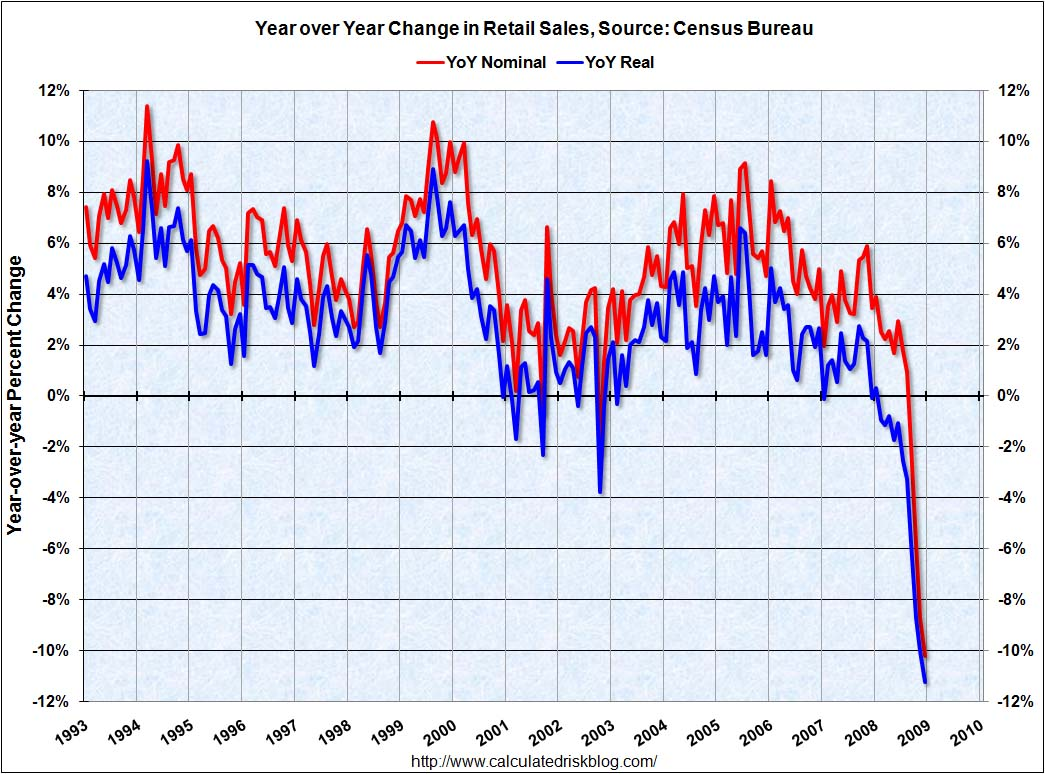
\includegraphics[width=3in]{/Volumes/Data/Code/ARK/PARKive/pri/PARK-make/Intro-To-ARK/ForEconomists/Figures/Retail-Sales-Collapse.jpg}
    \end{center}
    
  \end{frame}

  \begin{frame}{From All-Day Fed Workshop ...}

    Of course `uncertainty' is fashionable right now
    \begin{itemize} \pause
    \item Susanto Basu
    \item Nick Bloom
    \item Larry Christiano (!)
    \item Steve Davis
    \item Ulrike Malmendier
    \item ...
    \end{itemize}

    \pause    ... because $C$ collapse vastly exceeds what can be explained by traditional macro variables (wealth, credit supply, ...)
    
  \end{frame}

  \begin{frame}{From All-Day Fed Workshop ...}

    It's a Quantitative Theory question:
    \bi
  \item {\it How Big} would increase in $\sigma_{\psi}^{2}$ need to be to generate {\it entire} observed $C$ collapse?
    \ei

    \pause
    \bi
  \item If answer is absurd, maybe we have to look elsewhere
    \ei
    
  \end{frame}

  \begin{frame}{From All-Day Fed Workshop ...}

    Exercise: 
    
    \bi
  \item Take \cite{cstwMPC} model in ARK
  \item Traditional calibration (from Carroll (1992)!) so hands are tied
  \item Ask `how much of an increase in $\sigma^{2}_{\psi}$ would explain entire $C$ collapse'?
    \ei

    \pause ... over to MNW!  
    
  \end{frame}
} % ifInclude
\GMUHideEnd
\PARKmakeHideEnd

\subsection{Where}
\begin{frame}
  \frametitle{Where Is It?}

  Browse without installing:
  \begin{itemize}
  \item Browse on our webpage at \EconARK
  \item Browse our code at \phantom{}\href{http://github.com/econ-ark}{http://github.com/econ-ark} 
  \item Browse our talks at \href{http://github.com/econ-ark}{http://github.com/econ-ark/PARK} 
  \item Browse our live \href{https://econ-ark.org/notebooks}{notebooks} 
  \end{itemize}
\end{frame}
% \end{comment}
\begin{frame}
  \frametitle{Installing It On Your Local Computer}

  \begin{itemize}
  \item You Need Python 2.7 (Python 3 target is  July)
  \item If you don't have Python 2.7 on your computer, install either:
    \begin{enumerate}
    \item \href{https://www.anaconda.com/download/}{Anaconda2} - adds many packages useful for scientific computing
    \item Python 2.7
      \begin{itemize}
      \item \href{https://www.python.org/downloads/release/python-2715/}{On Mac or Linux} to download and install it
      \item \href{http://docs.python-guide.org/en/latest/starting/install/win/}{On Windows}
      \item Install \href{https://jupyter.org/install}{Jupyter}
      \item Make sure you have \href{https://packaging.python.org/tutorials/installing-packages/}{\texttt{pip}} installed
      \end{itemize}
    \item Install the `econ-ark' package:
      \begin{itemize}
      \item \texttt{pip install econ-ark}
      \end{itemize}
    \end{enumerate}
  \item  \pause Get our \href{http://econ-ark.org/notebooks}{our demonstration notebooks} from 
  \end{itemize}
\end{frame}


% People who haven't used pip before should download:

% https://files.pythonhosted.org/packages/40/e2/fd0ba9890096ee839583e378fdff408363a040c117bac89b8867e46ea9aa/econ-ark-0.8.0.dev3.tar.gz

% URLs to access:

% https://github.com/econ-ark/DemARK/

% https://mybinder.org/v2/gh/econ-ark/DemARK/master


% 



% \ifInclude{
\beamerdefaultoverlayspecification{<*>}
% }{}


\begin{frame}[t,allowframebreaks]
  \frametitle{References}
  \tiny 
  \input econtexBibMake
\end{frame}
\pagebreak

\end{document}


\CESifoHideBegin
\item \texttt{{\EconARK}/HARK/Documentation/NARK.pdf}
  \begin{itemize}
  \item Describes variable naming conventions for easy workflow: 
  \item LaTeX object definitions correspond to HARK definitions 
  \end{itemize}
\item Similar structure will be used for future contributions
  \begin{itemize}
  \item {\bf A}gent {\bf A}rchive {\bf R}epository {\bf D}eposit {\bf V}ehicle for ARK?
  \end{itemize}
  \CDSifoHideEnd
\item Instructions for cloning are in the README.txt
\item You get the whole codebase under the Apache license 
  \begin{itemize}
  \item Basically, no limitations on use
  \item But, please credit us, and participate in discussions
  \end{itemize}
\end{enumerate}

\end{frame}


\begin{frame}
  \frametitle{Organization Going Forward}

  Standard Github tools, esp:
  \begin{itemize}
  \item Issue Tracker: If You See Something, Say Something
  \end{itemize}
  \begin{center}
    {\bf Topic Czars}

    \begin{itemize}
    \item Gatekeeper for Contributions
    \item Responsible for Setting Out Tests A Module Should Pass
      \begin{itemize}
      \item e.g.\ Special Cases With Analytical Solutions
      \item Metrics for ``closeness'' to ``true'' solution
      \end{itemize}
    \end{itemize}

    \pause 
    \begin{tabular}{lll}
      Name & Topic & Affiliation
      \\ \hline  Serguei Maliar & Interpolation & Stanford %& \href{mailto:ccarroll@llorracc.org}{ccarroll@llorracc.org}
      \\ Lilia Maliar & Interpolation & Stanford % & \href{}{mailto:ccarroll@llorracc.org}
      \\  \multicolumn{3}{c}{{\it We're Seeking Volunteers for Czars}}
    \end{tabular}
  \end{center}

  \pause
  \begin{tabular}{rcl}
    \hline \href{mailto:info@econ-ark.org}{info@econ-ark.org} & - & General Purpose Questions
    \\ \href{mailto:czars@econ-ark.org}{czars@econ-ark.org} & - & Volunteer to be a Czar
    \\ \href{mailto:ideas@econ-ark.org}{ideas@econ-ark.org} & - & Ideas for Improvement
  \end{tabular}


\end{frame}


\begin{frame}
  \frametitle{Join our (Scientific) Revolution!}

  \providecommand{\subscribe}{\href{mailto:subscribe@econ-ark.org}{subscribe@econ-ark.org}}
  \providecommand{\letmehelpwith}{\href{mailto:letmehelpwith@econ-ark.org}{letmehelpwith@econ-ark.org}}
  Options:
  \begin{itemize}
  \item \subscribe
    \begin{itemize}
    \item Add me to the newsletter/mailing list
    \end{itemize}
  \item {\it Read the docs and slides} and absorb what exists now.  Options:
    \begin{enumerate}
    \item Add an `issue' that you want to tackle on \EconARK
    \item \letmehelpwith
      \begin{enumerate}
      \item Define some area that you'd like to contribute to
      \item email us at this address outlining what you propose to do
      \item We'll reply with some suggestions
      \end{enumerate}
    \end{enumerate}
  \end{itemize}

\end{frame}



\end{document}

\subsection{When}

\begin{frame}
  \frametitle{Timeline}

  \begin{center}
    \begin{tabular}{rll}
      When & What & Lessons
      \\ \hline 2006-2013 & \href{http://econ.jhu.edu/people/ccarroll/SolvingMicroDSOPs}{SolvingMicroDSOPs} & Surprisingly popular
      \\ 2014-12 & \href{}{IMF-CFPB Workshop} & Lots of enthusiasm
      \\ 2015-12 & \href{}{CFPB-IMF Workshop} & Not HARK, ARK!  
      \\ & & Testing, Replication, Feedback
      \\ 2016-06 & Hello! & None yet ...
    \end{tabular}
  \end{center}

  \begin{itemize}
  \item The version at \href{github.com/econ-ark}{http://github.com/econ-ark}  is our ``public beta''
  \item So far as we know, everything works
  \item First non-beta: Built-in tests for {\it everything}
    \begin{itemize}
    \item Aim: This year
    \end{itemize}
  \end{itemize}

\end{frame}



% \PARKmakeHideBegin
\ifInclude{
  \begin{frame}
    \frametitle{LATE is Antedeluvian}
    `Local Average Treatment Effects' results are 
    \begin{itemize}
    \item {\bf N}ot {\bf E}ven {\bf V}ery {\bf E}mpirically {\bf R}elevant ...
    \item UNLESS used to estimate `structural' parameters
    \item Because the important question is
      \begin{itemize}
      \item What does world look like {\it non-locally} ...
      \item ... = {\it after} the policy change
      \item and maybe not even just ``on average''
        \begin{itemize}
        \item because distributional/targeted impact may be whole point
        \end{itemize}
      \end{itemize}
    \end{itemize}
  \end{frame}
}
% \PARKmakeHideEnd

\begin{frame}
  \frametitle{Economists are People Too ...}

  \begin{itemize}
  \item We are {\it way} behind many scientific fields in `open source' code
  \item Surveys/Experiments: Economics students are more `selfish.'
  \item Options: \pause
    \begin{enumerate}
    \item `selfish' people study economics
    \item Studying economics makes you selfish!
    \item Economics students are just more honest
    \end{enumerate}
  \end{itemize}

  \pause I prefer (3)!

\end{frame}

\begin{frame}
  \frametitle{Lessons Learned from Other Fields About What Works}

  \begin{itemize}
  \item Not taking the dewy-eyed view: ``Build it and they will come''
  \item Emprical fact: Many other open source communities have succeeded
  \item Economists can't be {\it that} different ...
  \end{itemize}

\end{frame}

\begin{frame}
  \frametitle{In Addition to Usual Github Tools}

  \begin{itemize}
  \item Czars for specific topics
  \item Bounties for Best Solution of Specific Problems
  \item Time-Stamped Public Mechanism for Staking a Claim to New Idea
  \item Stack-Exchange-Like Q\&A Forum
  \item Mechanism for Easy Creation of Grad Student Problem Sets
  \item Tool for Grad Student Replication Exercises
  \item Eventually, a Journal?
  \item ... Your Ideas?  \href{mailto:ideas@econ-ark.org}{ideas@econ-ark.org}
  \end{itemize}

\end{frame}

\ifInclude{
  \begin{frame}\frametitle{Now: HA Structural Modeling Is Alchemy Not Chemistry}

    ... for outsiders: \pause Magic

    \bi \pause
  \item This is unfair: Alchemists {\it tried} to hide their methods 
    \ei
    
    \pause  Need to make it `normal science': \pause
    \bi
  \item Transparent, reproducible
  \item {\it easy} (not hard) to `stand on the shoulder of giants'
    \ei
  \end{frame}
} % ifInclude


